\documentclass[12pt]{article}

\usepackage{geometry}                % See geometry.pdf to learn the layout options. There are lots.
\usepackage{fullpage}
\usepackage{graphicx}
\usepackage{color, colortbl}
\usepackage{amsmath}
\usepackage{amssymb}
\usepackage{epstopdf}
\allowdisplaybreaks

\newcommand{\real}{{\mathbb{R}}}
\newcommand{\Id}{{\mathbb{I}}}
\newcommand{\xdot}{\dot{x}}
\newcommand{\eff}{\text{eff}}
\newcommand{\brug}{\text{brug}}
\providecommand{\sep}{\ensuremath{\rm{sep}}}
\newcommand{\pard}[2]{\frac{\partial #1}{\partial #2}}

\newcommand{\red}[1]{{\color{red}#1}}
\newcommand{\blue}[1]{{\color{blue}#1}}
\newcommand{\green}[1]{{\color{green}#1}}

\title{Numerical Implementation of the Doyle-Fuller-Newman (DFN) Model}
\author{{\normalsize Prof. Scott Moura} $\mid$ {\normalsize Energy, Controls, and Applications Lab (eCAL) $\mid$ UC Berkeley}}
\date{{\normalsize LAST UPDATED $\mid$ \today}}                                           % Activate to display a given date or no date

%%%%%%%%%%%%%%%%%%%%%%%%%%%
\begin{document}
\maketitle

%\section{}
%\subsection{}

In this note we document the numerical implementation of the DFN model.

%%%%%%%%%%%%%%%%%%%%%%%%%%%
\section{Doyle-Fuller-Newman Model}\label{sec:dfn}

We consider the Doyle-Fuller-Newman (DFN) model in Fig. \ref{fig:dfn-schematic} to predict the evolution of lithium concentration in the solid $c_{s}^{\pm}(x,r,t)$, lithium concentration in the electrolyte $c_{e}(x,t)$, solid electric potential $\phi_{s}^{\pm}(x,t)$, electrolyte electric potential $\phi_{e}(x,t)$, ionic current $i_{e}^{\pm}(x,t)$, molar ion fluxes $j_{n}^{\pm}(x,t)$, and bulk cell temperature $T(t)$ \cite{Thomas2002}. The governing equations are given by
\begin{eqnarray}
	\frac{\partial c_{s}^{\pm}}{\partial t}(x,r,t) &=& \frac{1}{r^{2}} \frac{\partial}{\partial r} \left[ D_{s}^{\pm} r^{2} \frac{\partial c_{s}^{\pm}}{\partial r}(x,r,t) \right], \label{eqn:cs} \\
	 \varepsilon_{e}^{j} \frac{\partial c_{e}^{j}}{\partial t}(x,t) &=& \frac{\partial}{\partial x} \left[D_{e}^{\text{eff}}(c_{e}^{j}) \frac{\partial c_{e}^{j}}{\partial x}(x,t) + \frac{1 - t_{c}^{0}}{F} i_{e}^{j}(x,t) \right], \ \label{eqn:ce} \\
	0 &=& \frac{\partial \phi_{s}^{\pm}}{\partial x}(x,t) - \frac{i_{e}^{\pm}(x,t) - I(t)}{\sigma^{\text{eff},\pm}}, \label{eqn:phis} \\
	0 &=& \kappa^{\text{eff}}(c_{e}) \cdot \frac{\partial \phi_{e}}{\partial x}(x,t) + i_{e}^{\pm}(x,t) \nonumber \\
	0 &=& \frac{\partial i_{e}^{\pm}}{\partial x}(x,t) - a_{s}^{\pm} F j_{n}^{\pm}(x,t), \label{eqn:ie} \\
	&& - \kappa^{\text{eff}}(c_{e}) \cdot \frac{2RT}{F}(1 - t_{c}^{0}) \times \left(1 + \frac{d \ln f_{c/a}}{d \ln c_{e}}(x,t) \right) \frac{\partial \ln c_{e}}{\partial x}(x,t), \label{eqn:phie}  \quad \\
	0 &=& \frac{1}{F} i_{0}^{\pm}(x,t) \left[e^{\frac{\alpha_{a}F}{RT} \eta^{\pm}(x,t)} - e^{-\frac{\alpha_{c}F}{RT} \eta^{\pm}(x,t)} \right] - j_{n}^{\pm}(x,t), \label{eqn:bv} \\
	\rho^{\textrm{avg}} c_{P} \frac{dT}{dt}(t) &=& h_{\textrm{cell}} \left[ T_{\textrm{amb}}(t) - T(t) \right] + I(t) V(t) -\int_{0^{-}}^{0^{+}} a_{s} F j_{n}(x,t) \Delta T(x,t) dx, \label{eqn:T}
\end{eqnarray}
where $D_{e}, \kappa, f_{c/a}$ are functions of $c_{e}(x,t)$ and \noindent $D_{e}^{\text{eff}} = D_{e}(c_{e}) \cdot (\varepsilon_{e}^{j})^{\text{brug}}$, $\sigma^{\text{eff}} = \sigma \cdot (\varepsilon_{s}^{j} + \varepsilon_{f}^{j})^{\text{brug}}$, $\kappa^{\text{eff}} = \kappa(c_{e}) \cdot (\varepsilon_{e}^{j})^{\text{brug}}$ are the effective electrolyte diffusivity, effective solid conductivity, and effective electrolyte conductivity given by the Bruggeman relationship. We also have
\begin{eqnarray}
	i_{0}^{\pm}(x,t) &=& k^{\pm}  \left[ c_{ss}^{\pm}(x,t) \right]^{\alpha_{c}} \left[c_{e}(x,t) \left(c_{s,\max}^{\pm} - c_{ss}^{\pm}(x,t)  \right) \right]^{\alpha_{a}}, \label{eqn:i0} \\
	\eta^{\pm}(x,t) &=& \phi_{s}^{\pm}(x,t) - \phi_{e}(x,t) - U^{\pm}(c_{ss}^{\pm}(x,t)) - F R_{f}^{\pm} j_{n}^{\pm}(x,t), \label{eqn:eta} \\
	c_{ss}^{\pm}(x,t) &=& c_{s}^{\pm}(x,R_{s}^{\pm},t), \label{eqn:css} \\
	\Delta T(x,t) &=& U^{\pm}(\overline{c}^{\pm}_{s}(x,t)) - T(t) \frac{\partial U^{\pm}}{\partial T}(\overline{c}^{\pm}_{s}(x,t)), \\
	\overline{c}_{s}^{\pm}(x,t) &=& \frac{3}{(R_{s}^{\pm})^{3}} \int_{0}^{R_{s}^{\pm}} r^{2} c_{s}^{\pm}(x,r,t) dr \label{eqn:cbulk}
\end{eqnarray}

\begin{figure}[t]
  \centering
  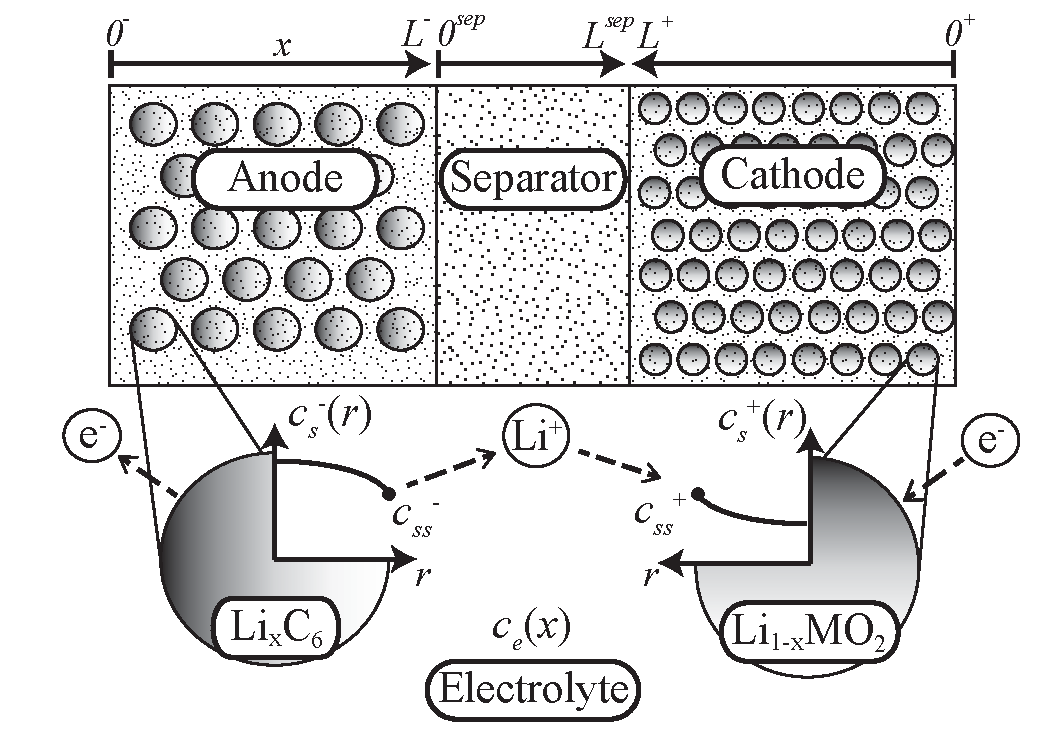
\includegraphics[trim = 0.4in 0.1in 0.15in 0.05in, clip, width=4.5in]{dfn-schematic.pdf}
  \caption{Schematic of the Doyle-Fuller-Newman model \cite{Thomas2002}. The model considers two phases: the solid and electrolyte. In the solid, states evolve in the $x$ and $r$ dimensions. In the electrolyte, states evolve in the $x$ dimension only. The cell is divided into three regions: anode, separator, and cathode.}
  \label{fig:dfn-schematic}
\end{figure}

Along with these equations are corresponding boundary and initial conditions. The boundary conditions for the solid-phase diffusion PDE (\ref{eqn:cs}) are
\begin{eqnarray}
	\frac{\partial c_{s}^{\pm}}{\partial r}(x,0,t) &=& 0, \label{eqn:cs-bc1} \\
	\frac{\partial c_{s}^{\pm}}{\partial r}(x,R_{s}^{\pm},t) &=& -\frac{1}{D_{s}^{\pm}} j_{n}^{\pm} \label{eqn:cs-bc2}.
\end{eqnarray}
The boundary conditions for the electrolyte-phase diffusion PDE (\ref{eqn:ce}) are given by
\begin{align}
	\pard{c_{e}}{x}(0^{-},t) &= \pard{c_{e}}{x}(0^{+},t) = 0, \label{eqn:ce-bc1} \\
	\varepsilon_{e}^{-} D_{e}^{-}(L^{-}) \pard{c_{e}}{x}(L^{-},t) &= \varepsilon_{e}^{\textrm{sep}}D_{e}^{\textrm{sep}}(0^{\textrm{sep}}) \pard{c_{e}}{x}(0^{\textrm{sep}},t), \\
	\varepsilon_{e}^{\textrm{sep}}D_{e}^{\textrm{sep}}(L^{\textrm{sep}}) \pard{c_{e}}{x}(L^{\textrm{sep}},t) &= \varepsilon_{e}^{+} D_{e}^{+}(L^{+}) \pard{c_{e}}{x}(L^{+},t), \\
	c_{e}(L^{-},t) &= c_{e}(0^{\textrm{sep}},t), \\
	c_{e}(L^{\textrm{sep}},t) &= c_{e}(0^+,t). \label{eqn:ce-bc5}
\end{align}
The boundary conditions for the solid-phase potential ODE (\ref{eqn:phis}) are given by
\begin{equation}\label{eqn:phis-bc}
	\pard{\phi_{s}^{-}}{x}(L^{-},t) = \pard{\phi_{s}^{+}}{x}(L^{+},t) = 0.
\end{equation}
The boundary conditions for the electrolyte-phase potential ODE (\ref{eqn:phie}) are given by
\begin{eqnarray}
	\phi_{e}(0^{-},t) &=& 0, \\
	\phi_{e}(L^{-},t) &=& \phi_{e}(0^{\textrm{sep}},t), \\
	\phi_{e}(L^{\textrm{sep}},t) &=& \phi_{e}(L^+,t).
\end{eqnarray}
The boundary conditions for the ionic current ODE (\ref{eqn:ie}) are given by
\begin{equation}\label{eqn:ie-bcs}
	i_{e}^{-}(0^{-},t) = i_{e}^{+}(0^+,t) = 0
\end{equation}
and also note that $i_{e}(x,t) = I(t)$ for $x \in [0^{\textrm{sep}}, L^{\textrm{sep}}]$.

In addition, the parameters $D_s^{\pm}, D_e, \kappa_e, k^{\pm}$ vary with temperature via the Arrhenius relationship:
\begin{equation}\label{eqn:arrhenius}
	\psi = \psi_{ref} \exp \left[\frac{E_\psi}{R} \left( \frac{1}{T} - \frac{1}{T_{ref}} \right) \right]
\end{equation}
where $\psi$ represents a temperature dependent parameter, $E_{\psi}$ is the activation energy [J/mol], and $\psi_{ref}$ is the reference parameter value at reference temperature $T_{ref}$.

The input to the model is the applied current density  $I(t)$ [A/m$^{2}$], and the output is the voltage measured across the current collectors
\begin{equation}\label{eqn:voltage}
	V(t) = \phi^{+}_{s}(0^{+},t) - \phi_{s}^{-}(0^{-},t) - R_c I(t)
\end{equation}
Further details, including notation definitions, can be found in \cite{Thomas2002,Chaturvedi2010}.

%%%%%%%%%%%%%%%%%%%%%%%%%%%
\section{Time-stepping}\label{sec:time-step}

Ultimately, the equations are discretized to produce a DAE in the following format:
\begin{eqnarray}
	\xdot &=& f(x, z, u), \label{eqn:dae1} \\
	0 &=& g(x,z,u) \label{eqn:dae2}
\end{eqnarray}
with initial conditions $x(0), z(0)$ that are consistent. That is, they verify (\ref{eqn:dae2}). The time-stepping is done by solving the nonlinear equation
\begin{align}
	 0 &= F(x(t + \Delta t), z(t + \Delta t)), \label{eqn:cfn1} \\
0 &= \left[
\begin{array}{c}
  x(t) - x(t+\Delta t) + \frac{1}{2} \Delta t \left[ f(x(t), z(t), u(t)) + f(x(t+\Delta t), z(t+\Delta t), u(t+\Delta t)) \right] \\
  g\left(x(t+\Delta t), z(t+\Delta t), u(t + \Delta t) \right)
\end{array}
\right] \label{eqn:cfn2}
\end{align} 
for $x(t+\Delta t), z(t+\Delta t)$. The function \texttt{cfn\_dfn.m} returns the solution $\left(x(t+\Delta t), z(t+\Delta t)\right)$ of (\ref{eqn:cfn1})-(\ref{eqn:cfn2}), given $x(t), z(t), u(t), u(t+\Delta t)$. Note that we solve (\ref{eqn:cfn1})-(\ref{eqn:cfn2}) using Newton's method, meaning analytic Jacobians of $F(\cdot, \cdot)$ are required w.r.t. $x,z$.
\begin{align}
J &=
\left[
\begin{array}{cc}
 F^{1}_{x} & F^{1}_{z}  \\
 F^{2}_{x} & F^{2}_{z}
\end{array}
\right] \\
&= 
\left[
\begin{array}{cc}
 -I + \frac{1}{2} \Delta t \cdot \frac{\partial f}{\partial x}(x(t+\Delta t),z(t+\Delta t),u(t+\Delta t)) & \frac{1}{2} \Delta t \cdot \frac{\partial f}{\partial z}(x(t+\Delta t),z(t+\Delta t),u(t+\Delta t))  \\
 \frac{\partial g}{\partial x}(x(t+\Delta t),z(t+\Delta t),u(t+\Delta t)) & \frac{\partial g}{\partial z}(x(t+\Delta t),z(t+\Delta t),u(t+\Delta t))
\end{array}
\right]
\end{align}
The analytic Jacobian is computed in two functions: (i) Function \texttt{jac\_dfn\_pre.m} computes Jacobian elements that are NOT state/time-dependent. (ii) Function \texttt{jac\_dfn.m} computes Jacobian elements that are state/time-dependent.

%%%%%%%%%%%%%%%%%%%%%%%%%%%
\section{DAEs}\label{sec:daes}
To perform the time-stepping in the previous section, we must compute functions $f(x,z,u)$ and $g(x,z,u)$. These functions, which represent the RHS of (\ref{eqn:dae1})-(\ref{eqn:dae2}), are calculated by the Matlab function \texttt{dae\_dfn.m}, given the inputs $x,z,u$. The role of variables $x,z,u$ are played by the DFN variables shown in Table \ref{tbl:dae-notation}.

\begin{table}[h]
\caption{DAE notation for DFN states in Matlab Code}
\begin{center}
\begin{tabular}{c|c}
\hline \hline
\textbf{DAE Variable} & \textbf{DFN Variable} \\
\hline
$x$ & $c_{s}^{-}, c_{s}^{+}, c_{e} = [c_{e}^{-}, c_{e}^{sep}, c_{e}^{+}], T$ \\
$z$ & $\phi_{s}^{-}, \phi_{s}^{+}, i_{e}^{-}, i_{e}^{+}, \phi_{e} = [\phi_{e}^{-}, \phi_{e}^{sep}, \phi_{e}^{+}], j_{n}^{-}, j_{p}^{+}$ \\
$u$ & $I$ \\
\hline \hline
\end{tabular}
\end{center}
\label{tbl:dae-notation}
\end{table}%

In the subsequent sections, we go through each DFN variable listed in Table \ref{tbl:dae-notation} and document its numerical implementation.

%%%%%%%%%%%%%%%%%%%%%%%%%%%
\section{Solid Concentration, $c_{s}^{-}, c_{s}^{+}$}\label{sec:cs}
\green{[DONE]} The PDEs (\ref{eqn:cs}) and BCs (\ref{eqn:cs-bc1})-(\ref{eqn:cs-bc2}) governing Fickian diffusion in the solid phase are implemented using third order Pad\'{e} approximations of the transfer function from $j_{n}^{\pm}$ to $c_{ss}^{\pm}$ \cite{Forman2011a,Rahn2012}: 
\begin{equation}
	\frac{C_{ss}^{\pm}(s)}{J_{n}^{\pm}(s)} = \frac{-\frac{(R_{s}^{\pm})^3}{165 (D_{s}^{\pm})^2}s^{2} -\frac{4 R_{s}^{\pm}}{11 D_{s}^{\pm}}s -\frac{3}{R_{s}^{\pm} }  }{ \frac{(R_s^{\pm})^4}{3465}s^3 + \frac{3 (R_s^{\pm})^2}{55 D_s^{\pm}}s^2 + s },
\end{equation}
which we notate more simply by
\begin{equation}
	\frac{C_{ss}^{\pm}(s)}{J_{n}^{\pm}(s)} = \frac{b_2 s^{2} + b_1 s + b_0 }{ a_3 s^3 + a_2 s^2 + a_1 s + a_0 }.
\end{equation}
Next we multiply top and bottom by $\frac{1}{a_3}$ to yield a unity coefficient on the highest-order term in the denominator, yielding
\begin{equation}\label{eqn:cs-tf}
	\frac{C_{ss}^{\pm}(s)}{J_{n}^{\pm}(s)} = \frac{\bar{b}_2 s^{2} + \bar{b}_1 s + \bar{b}_0 }{ s^3 + \bar{a}_2 s^2 + \bar{a}_1 s + \bar{a}_0 },
\end{equation}
where $\bar{b}_i = b_i/a_3$ and $\bar{a}_i = a_i/a_3$.

%\begin{eqnarray}
%	\frac{C_{ss}^{\pm}(s)}{J_{n}^{\pm}(s)} &=& \frac{-\frac{21}{R_{s}^{\pm}}s^{2} -\frac{1260 D_{s}^{\pm}}{(R_{s}^{\pm})^{3}}s -\frac{10395 (D_{s}^{\pm})^{2}}{ (R_{s}^{\pm})^{4} }  }{s^{3} + \frac{189 D_{s}^{\pm}}{(R_{s}^{\pm})^{2}} s^{2} + \frac{3465 (D_{s}^{\pm})^{2}}{(R_{s}^{\pm})^{4}} s }, \\
%	\frac{\overline{C}_{s}^{\pm}(s)}{J_{n}^{\pm}(s)} &=& \frac{-3 R_{s}^{\pm}}{s}.
%\end{eqnarray}
The transfer function (\ref{eqn:cs-tf}) is converted into controllable canonical state-space form, thus producing the subsystem:
\begin{eqnarray}
\frac{d}{dt}
\left[
\begin{array}{c}
 c_{s1}^{\pm}(t) \\
 c_{s2}^{\pm}(t) \\
 c_{s3}^{\pm}(t)
\end{array}
\right]
&=&
\left[
\begin{array}{ccc}
 0 & 1  & 0  \\
 0 & 0  & 1  \\
 -\bar{a}_0 & -\bar{a}_1  & -\bar{a}_2  
\end{array}
\right]
\left[
\begin{array}{c}
 c_{s1}^{\pm}(t) \\
 c_{s2}^{\pm}(t) \\
 c_{s3}^{\pm}(t)
\end{array}
\right] + 
\left[
\begin{array}{c}
 0 \\
 0 \\
 1
\end{array} \label{eqn:cs-ss-cc1}
\right] j_{n}^{\pm}(t) \\
\left[
\begin{array}{c}
 c_{ss}^{\pm}(t) \\
\end{array}
\right] &=& 
\left[
\begin{array}{ccc}
 \bar{b}_0 & \bar{b}_1  & \bar{b}_2
\end{array}
\right]
\left[
\begin{array}{c}
 c_{s1}^{\pm}(t) \\
 c_{s2}^{\pm}(t) \\
 c_{s3}^{\pm}(t)
\end{array}
\right] \label{eqn:cs-ss-cc2}
\end{eqnarray}
for each discrete point in $x$.

To simplify analytical applications for the DFN model, we seek a different state-space realization in which bulk concentration $\bar{c}_s^{\pm}(t)$ is expressed as a state. This can be found by pursuing a Jordan-form state-space realization, which diagonalizes the system matrix. The diagonal elements represent the system eigenvalues. The zero eigenvalue corresponds to bulk concentration. All the aforementioned calculations are performed in Matlab function \texttt{c\_s\_mats.m}. The final result produces system matrices:
\begin{eqnarray}
\frac{d}{dt}
\left[
\begin{array}{c}
 c_{s1}^{\pm}(t) \\
 c_{s2}^{\pm}(t) \\
 c_{s3}^{\pm}(t)
\end{array}
\right]
&=&
A_{cs}^{\pm}
\left[
\begin{array}{c}
 c_{s1}^{\pm}(t) \\
 c_{s2}^{\pm}(t) \\
 c_{s3}^{\pm}(t)
\end{array}
\right] + 
B_{cs}^{\pm} \ j_{n}^{\pm}(t) \label{eqn:cs-ss-jordan1} \\
\left[
\begin{array}{c}
 c_{ss}^{\pm}(t) \\
 \bar{c}_s^{\pm}(t)
\end{array}
\right] &=& 
C_{cs}^{\pm}
\left[
\begin{array}{c}
 c_{s1}^{\pm}(t) \\
 c_{s2}^{\pm}(t) \\
 c_{s3}^{\pm}(t)
\end{array}
\right] \label{eqn:cs-ss-jordan2}
\end{eqnarray}
where the second row of $C_{cs}^{\pm}$ is $[C_{cs}^{\pm}]_2 = [0, 0, 1]$. Note we have abused notation. The states in (\ref{eqn:cs-ss-jordan1})-(\ref{eqn:cs-ss-jordan2}) are not the same as those in (\ref{eqn:cs-ss-cc1})-(\ref{eqn:cs-ss-cc2}), due to the different realizations. Also, these matrices must be computed online, due to the temperature dependence of $D_s^{\pm}$ described in (\ref{eqn:arrhenius}).

%%%%%%%%%%%%%%%%%%%%%%%%%%%
\section{Electrolyte Concentration, $c_{e}$}\label{sec:ce}
\green{[DONE]} The electrolyte concentration PDE (\ref{eqn:ce}) combined with (\ref{eqn:ie}), and BCs (\ref{eqn:ce-bc1})-(\ref{eqn:ce-bc5}) are implemented using the central difference method, which ultimately produces the matrix differential equation:
\begin{equation}
	\frac{d}{dt} c_{e}^j(t) = \frac{d D_e^{\eff,j}}{d c_e}(c_e^j) \left[ M^{j,1}_{ce} c_{e}^j(t) + M^{j,2}_{ce} c_{e,bc}^j(t) \right]^2 + D_e^{\eff,j}(c_e^j) \left[ M^{j,3}_{ce} c_{e}^j(t) + M^{j,4}_{ce} c_{e,bc}^j(t) \right] + M^{j,5}_{ce} j_{n}^j(t)
\end{equation}
where $c_{e}, j_{n}^j$ are vectors whose elements represent discrete points along the $x$-dimension of the DFN model. The variable $c_{e,bc}^j$ represents the boundary values for region $j$, namely $c_{e,bc}^- = \left[c_{e,bc,1}, c_{e,bc,2} \right]^T$, $c_{e,bc}^{\sep} = \left[c_{e,bc,2}, c_{e,bc,3} \right]^T$, $c_{e,bc}^{+} = \left[c_{e,bc,3}, c_{e,bc,4} \right]^T$. The boundary values are computed by: $c_{e,bc}(t) = C_{ce} \ c_{e}(t)$ where $c_{e,bc} = \left[c_{e,bc,1}, c_{e,bc,2}, c_{e,bc,3}, c_{e,bc,4} \right]^T$.

%Note that $i_{e,x}$ and $c_{e,x}$ represent the entire electrolyte current and concentration, respectively, across the entire battery, including boundary values,
%\begin{eqnarray}
%	i_{e,x}(t) &=& \left[0, \ i_{e}^{-}(x,t), \ I(x,t), \ i_{e}^{+}(x,t), \ 0 \right]^{T}, \label{eqn:iex} \\
%	c_{e,x}(t) &=& \left[c_{e,bc,1}(t), \ c_{e}^{-}(x,t), c_{e,bc,2}(t), \ c_{e}^{sep}(x,t), c_{e,bc,3}(t), \ c_{e}^{+}(x,t), \ c_{e,bc,4}(t) \right]^{T}, \label{eqn:cex} \\ 
%	c_{e,bc}(t) &=& C_{ce} \ c_{e}(t) 
%\end{eqnarray}
Note that the effective diffusivity, $D_e^{\eff,j}(c_e^j)$, and its derivative, $\frac{d D_e^{\eff,j}}{d c_e}(c_e^j)$, are state-dependent and must be computed online. The matrices $M^{j,1}_{ce}, M^{j,2}_{ce}, M^{j,3}_{ce}, M^{j,4}_{ce}, M^{j,5}_{ce}, C_{ce}$ are computed offline by Matlab function \texttt{c\_e\_mats.m}. These matrices are given by
\begin{align}
M^{j,1}_{ce} &=
\frac{1}{2 L^j \Delta x^j} \left[
\begin{array}{ccccc}
 0 & 1 & 0 & \ldots & 0  \\
 -1 & 0 & 1 & \ldots & 0  \\
 0 & -1 & 0 & \ldots & 0  \\
 \vdots & \vdots & \vdots &  &  \\
 0 & 0 & \cdots & \cdots & 1 \\
 0 & 0 & \cdots & -1 & 0 \\
\end{array}
\right], \quad
M^{j,2}_{ce} =
\frac{1}{2 L^j \Delta x^j} \left[
\begin{array}{cc}
 -1 & 0  \\
 0 & 0 \\
 \vdots & \vdots  \\
 0 & 0 \\
 0 & 1 \\
\end{array}
\right], \qquad \\
M^{j,3}_{ce} &= \frac{1}{(L^j \Delta x^j)^2}
\left[
\begin{array}{cccccc}
 1 & -2 & 1 & \ldots & & 0  \\
 0 & 1 & -2 & \ldots & & 0  \\
 \vdots & \vdots & \vdots & & & \vdots \\
 0 & 0 & \cdots & 1 & -2 & 1 \\
 0 & 0 & \cdots & 0 & 1 & -2 \\
\end{array}
\right], \quad
M^{j,4}_{ce} =
\frac{1}{(L^j \Delta x^j)^2} \left[
\begin{array}{cc}
 1 & 0  \\
 0 & 0 \\
 \vdots & \vdots  \\
 0 & 0 \\
 0 & 1 \\
\end{array}
\right], \qquad \\
M^{j,5}_{ce} &= \frac{(1-t_c^0)a_s^j}{\varepsilon_e^j}
\mathbb{I}.
\end{align}
for $j \in \{-,\sep,+\}$. The matrix $C_{ce}$ is given by
\begin{equation}
	C_{ce} = -(N^2_{ce})^{-1}(N^1_{ce})
\end{equation}
where
\begin{eqnarray}
	N^1_{ce} &=& 
        \left[
        \begin{array}{ccccc|ccc}
         4 & -1 & \cdots & 0 & 0 & 0 & 0 & \cdots \\
         0 & 0 & \cdots & \frac{(\varepsilon_e^-)^{\brug}}{2L^- \Delta x^-} & -4 \frac{(\varepsilon_e^-)^{\brug}}{2L^- \Delta x^-} & -4 \frac{(\varepsilon_e^{\sep})^{\brug}}{2L^{\sep} \Delta x^{\sep}} &  \frac{(\varepsilon_e^{\sep})^{\brug}}{2L^{\sep} \Delta x^{\sep}} & \cdots \\
         4 & 0 & \cdots & 0 & 0 & 0 & 0 & \cdots \\
         0 & 0 & \cdots & 0 & 0 & 0 & 0 & \cdots 
        \end{array}
        \right. \nonumber \\
        && \left.
        \begin{array}{ccc|ccccc}
        \cdots & 0 & 0 & 0 & 0 & \cdots & 0 & 0 \\
        \cdots & 0 & 0 & 0 & 0 & \cdots & 0 & 0 \\
        \cdots & \frac{(\varepsilon_e^{\sep})^{\brug}}{2L^{\sep} \Delta x^{\sep}} & -4 \frac{(\varepsilon_e^{\sep})^{\brug}}{2L^{\sep} \Delta x^{\sep}} & -4 \frac{(\varepsilon_e^{+})^{\brug}}{2L^{+} \Delta x^{+}} & \frac{(\varepsilon_e^{+})^{\brug}}{2L^{+} \Delta x^{+}} & \cdots & 0 & 0 \\
        \cdots & 0 & 0 & 0 & 0 & \cdots & 1 & -4
        \end{array}
        \right] \\
	N^2_{ce} &=& 
        \left[
        \begin{array}{cccc}
        -3  &  0 & 0 & 0 \\
         0  &  3\frac{(\varepsilon_e^-)^{\brug}}{2L^- \Delta x^-} + 3 \frac{(\varepsilon_e^{\sep})^{\brug}}{2L^{\sep} \Delta x^{\sep}} & 0 & 0 \\
         0 & 0  & 3 \frac{(\varepsilon_e^{\sep})^{\brug}}{2L^{\sep} \Delta x^{\sep}} + 3\frac{(\varepsilon_e^+)^{\brug}}{2L^+ \Delta x^+}& 0 \\
        0 & 0  & 0 & 3 
        \end{array}
        \right].
\end{eqnarray}
Note, we have used second-order accurate finite difference approximations for the boundary conditions.

%\clearpage
%\begin{eqnarray}
%	A_{ce} &=& (M1) - (M2) (N2)^{-1} (N1), \\ 
%	B_{ce} &=& (M3), \\
%	C_{ce} &=& - (N2)^{-1} (N1)
%\end{eqnarray}
%The first term on the RHS of PDE (\ref{eqn:ce}) is implemented by
%\begin{eqnarray}
%	(M1) &=& \textrm{BlkDiag}\left( (M1n), (M1s), (M1p) \right), \\
%	(M2) &=&
%\left[
%\begin{array}{cccc}
% (M2n_{col1}) & (M2n_{col2}) & 0 & 0 \\
% 0 & (M2s_{col1}) & (M2s_{col2}) & 0 \\
% 0 & 0 & (M2p_{col1}) & (M2p_{col2}) \\
%\end{array}
%\right]
%\end{eqnarray}
%and
%\begin{align}
%&(M1n) =  \nonumber \\
%&\alpha^{-} \cdot \left[
%\begin{array}{cccc}
%  -(D_{e,0} + D_{e,n,2}) & D_{e,n,2}  &  & \\
%  D_{e,n,1} & -(D_{e,n,1}+D_{e,n,3})  & D_{e,n,3} & \\
%  \ddots & \ddots  & \ddots & \\
%  & D_{e,n,i-1} & -(D_{e,n,i-1} + D_{e,n,i+1}) & D_{e,n,i+1} \\
%  & \ddots & \ddots  & \ddots \\
%%  &   & D_{e,n,Nxn-1} & -(D_{e,n,Nxn-3} + D_{e,n,Nxn-1}) & D_{e,n,Nxn-1} \\
%  &  & D_{e,n,Nxn-2} & -(D_{e,n,Nxn-2} + D_{e,ns})
%\end{array}
%\right]
%\end{align}
%\begin{align}
%&(M1s) =  \nonumber \\
%&\alpha^{sep} \cdot \left[
%\begin{array}{cccc}
%  -(D_{e,ns} + D_{e,s,2}) & D_{e,s,2}  &  & \\
%  D_{e,s,1} & -(D_{e,s,1}+D_{e,s,3})  & D_{e,s,3} & \\
%  \ddots & \ddots  & \ddots & \\
%  & D_{e,s,i-1} & -(D_{e,s,i-1} + D_{e,s,i+1}) & D_{e,s,i+1} \\
%  & \ddots & \ddots  & \ddots \\
%%  &   & D_{e,n,Nxn-1} & -(D_{e,n,Nxn-3} + D_{e,n,Nxn-1}) & D_{e,n,Nxn-1} \\
%  &  & D_{e,s,Nxs-2} & -(D_{e,s,Nxs-2} + D_{e,np})
%\end{array}
%\right]
%\end{align}
%\begin{align}
%&(M1p) =  \nonumber \\
%&\alpha^{+} \cdot \left[
%\begin{array}{cccc}
%  -(D_{e,sp} + D_{e,p,2}) & D_{e,p,2}  &  & \\
%  D_{e,p,1} & -(D_{e,p,1}+D_{e,p,3})  & D_{e,p,3} & \\
%  \ddots & \ddots  & \ddots & \\
%  & D_{e,p,i-1} & -(D_{e,p,i-1} + D_{e,p,i+1}) & D_{e,p,i+1} \\
%  & \ddots & \ddots  & \ddots \\
%%  &   & D_{e,n,Nxn-1} & -(D_{e,n,Nxn-3} + D_{e,n,Nxn-1}) & D_{e,n,Nxn-1} \\
%  &  & D_{e,p,Nxp-2} & -(D_{e,p,Nxp-2} + D_{e,N})
%\end{array}
%\right]
%\end{align}
%\begin{equation}
%(M2n) = 
%\alpha^{-} \left[
%\begin{array}{cc}
%  D_{e,0} & 0 \\
%  0 & 0 \\
%  \vdots & \vdots \\
%  0 & D_{e,ns} \\
%\end{array}
%\right], \
%(M2s) = 
%\alpha^{sep} \left[
%\begin{array}{cc}
%  D_{e,ns} & 0 \\
%  0 & 0 \\
%  \vdots & \vdots \\
%  0 & D_{e,sp} \\
%\end{array}
%\right], \
%(M2p) = 
%\alpha^{+} \left[
%\begin{array}{cc}
%  D_{e,sp} & 0 \\
%  0 & 0 \\
%  \vdots & \vdots \\
%  0 & D_{e,N} \\
%\end{array}
%\right]
%\end{equation}
%\begin{equation}
%(M3) = 
%\left[
%\begin{array}{cccc |c| ccc |c| cccc}
%  -\beta^{-} & 0 & \beta^{-} &  &  &  &  &  &  &  &  &  &  \\
%   & \ddots & \ddots & \ddots &  &  &  &  &  &  &  &  &  \\
%   &  & -\beta^{-} & 0 & \beta^{-} &  &  &  &  &  &  &  &  \\
%   \hline
%   &  &  &  & -\beta^{sep} &  0 &  \beta^{sep}  &  &  &  &  &  &  \\
%   &  &  &  &  & \ddots & \ddots & \ddots &  &  &  &  &  \\
%   &  &  &  &  &  & -\beta^{sep} & 0 & \beta^{sep} &  &  &  &  \\
%   \hline
%   &  &  &  &  & &  &   & -\beta^{+} & 0 & \beta^{+} &  &  \\
%   &  &  &  &  & &  &   &  & \ddots & \ddots & \ddots &  \\
%   &  &  &  &  & &  &   &  &  & -\beta^{+} & 0 & \beta^{+} \\
%\end{array}
%\right]
%\end{equation}
%
%and
%\begin{eqnarray}
%	\alpha^{j} &=& \frac{1}{\left(L^{j} \Delta x^{j} \right)^{2}}, \qquad \beta^{j} = \frac{1 - t_{c}^{0}}{2 \varepsilon_{e}^{j} F L^{j} \Delta x^{j}}, \\
%	D_{e}(c_{e,x}(x,t)) &=& \left[ D_{e,0} \mid D_{e,n}(x) \mid D_{e,ns} \mid D_{e,s}(x) \mid D_{e,sp} \mid D_{e,p}(x) \mid D_{e,N} \right]
%\end{eqnarray}
%
%
%The boundary conditions (\ref{eqn:ce-bc1})-(\ref{eqn:ce-bc5}) are implemented as
%\begin{align}
%(N1) &=
%\left[
%\begin{array}{cccc | cccc | cccc}
%  \frac{1}{L^{-} \Delta x^{-}} & 0 & \cdots & 0 & 0 & \cdots & & 0 & 0 & \cdots & & 0\\
%  0 & \cdots & 0 & \frac{D_{e,ns}}{L^{-}\Delta x^{-}} & \frac{D_{e,ns}}{L^{sep}\Delta x^{sep}} & 0 & \cdots & 0 & 0 & \cdots & & 0\\
%  0 & 0 & \cdots & 0 & 0 & \cdots & 0 & \frac{D_{e,sp}}{L^{sep}\Delta x^{sep}} & \frac{D_{e,sp}}{L^{+}\Delta x^{+}} & 0 & \cdots & 0\\
%  0 & 0 & \cdots & 0 & 0 & \cdots & & 0 & 0 & \cdots & 0 & \frac{-1}{L^{+} \Delta x^{+}}
%\end{array}
%\right], \\
%(N2) &= 
%\left[
%\begin{array}{cccc}
%  \frac{-1}{L^{-} \Delta x^{-}} & 0  & 0 & 0 \\
%  0 & -\frac{D_{e,ns}}{L^{-} \Delta x^{-}} - \frac{D_{e,ns}}{L^{sep} \Delta x^{sep}}  & 0  & 0 \\
%  0 & 0  & -\frac{D_{e,sp}}{L^{sep} \Delta x^{sep}} - \frac{D_{e,sp}}{L^{+} \Delta x^{+}} & 0 \\
%  0 & 0  & 0  & \frac{1}{L^{+} \Delta x^{+}}
%\end{array}
%\right]
%\end{align}


%%%%%%%%%%%%%%%%%%%%%%%%%%%
\section{Temperature, $T$}\label{sec:T}
\green{[DONE]} Temperature is scalar, so the ODE (\ref{eqn:T}) is directly implemented as:
\begin{eqnarray}
\rho^{\textrm{avg}} c_{P} \frac{dT}{dt}(t) &=& h_{\textrm{cell}} \left[ T_{\textrm{amb}}(t) - T(t) \right] + I(t) V(t) -\int_{0^{-}}^{0^{+}} a_{s} F j_{n}(x,t) \Delta T(x,t) dx, \\
\Delta T(x,t) &=& U^{\pm}(\overline{c}^{\pm}_{s}(x,t)) - T(t) \frac{\partial U^{\pm}}{\partial T}(\overline{c}^{\pm}_{s}(x,t)), \\
\overline{c}_{s}^{\pm}(x,t) &=& \frac{3}{(R_{s}^{\pm})^{3}} \int_{0}^{R_{s}^{\pm}} r^{2} c_{s}^{\pm}(x,r,t) dr 
\end{eqnarray}

%%%%%%%%%%%%%%%%%%%%%%%%%%%
\section{Solid Potential, $\phi_{s}^{-}, \phi_{s}^{+}$}\label{sec:phis}
\green{[DONE]} The solid potential ODE (\ref{eqn:phis}) and BCs (\ref{eqn:phis-bc}) are implemented using the central difference method, which ultimately produces the matrix equation:
\begin{eqnarray}
	\frac{d}{dt} \phi_{s}^{-}(t) &=& F^{1}_{psn} \ \phi_{s}^{-}(t) + F^{2}_{psn} \ i_{e,aug}^{-}(t) + G_{psn} \ I(t) = 0 \\
	\frac{d}{dt} \phi_{s}^{+}(t) &=& F^{1}_{psp} \ \phi_{s}^{+}(t) + F^{2}_{psp} \ i_{e,aug}^{+}(t) + G_{psp} \ I(t) = 0.
\end{eqnarray}
where $i_{e,aug}^{\pm}$ are 
\begin{equation}\label{eqn:i_ex}
i_{e,aug}^{-}(t) = 
\left[
\begin{array}{c}
  0 \\
  i_{e}^{-}(x,t) \\
  I(t)
\end{array}
\right], \qquad
i_{e,aug}^{+}(t) = 
\left[
\begin{array}{c}
  I(t) \\
  i_{e}^{+}(x,t) \\
  0
\end{array}
\right]
\end{equation}
This section also computes the terminal voltage $V(t)$ from (\ref{eqn:voltage}) using matrix equations
\begin{eqnarray}
	\phi_{s,bc}^{-}(t) &=& C_{psn} \ \phi_{s}^{-}(t) + D_{psn} \ I(t), \\
	\phi_{s,bc}^{+}(t) &=& C_{psp} \ \phi_{s}^{+}(t) + D_{psp} \ I(t), \\
	V(t) &=& \phi_{s,bc,2}^{+}(t) - \phi_{s,bc,1}^{-}(t) - R_c I(t)
\end{eqnarray}
where the following matrices are computed a priori by Matlab function \texttt{phi\_s\_mats.m}
\begin{align}
	(F1n) &= (M1n) - (M2n) (N2n)^{-1} (N1n), \\
	(F2n) &= (M3n), \\
	(Gn) &= (M4n) - (M2n) (N2n)^{-1} (N3n), \\
	(F1p) &= (M1p) - (M2p)(N2p)^{-1}(N1p), \\
	(F2p) &= (M3p), \\
	(Gp) &= (M4p) - (M2p)(N2p)^{-1}(N3p), \\
	(Cn) &= -(N2n)^{-1}(N1n), \\
	(Dn) &= -(N2n)^{-1}(N3n), \\
	(Cp) &= -(N2p)^{-1}(N1p), \\
	(Dp) &= -(N2p)^{-1}(N3p),
\end{align}
where the $(Mij)$ and $N(ij)$ matrices result from central difference approximations of the ODE in space (\ref{eqn:phis}) and boundary conditions (\ref{eqn:phis-bc}).
\begin{align}
(M1j) &=
\left[
\begin{array}{ccccc}
 0 & \alpha_{j} & 0 & \ldots & 0  \\
 -\alpha_{j} & 0 & \alpha_{j} & \ldots & 0  \\
 0 & -\alpha_{j} & 0 & \ldots & 0  \\
 \vdots & \vdots & \vdots &  &  \\
 0 & 0 & \cdots & \cdots & \alpha_{j} \\
 0 & 0 & \cdots & -\alpha_{j} & 0 \\
\end{array}
\right], \quad
(M2j) =
\left[
\begin{array}{cc}
 -\alpha_{j} & 0  \\
 0 & 0 \\
 \vdots & \vdots  \\
 0 & 0 \\
 0 & \alpha_{j} \\
\end{array}
\right], \qquad \\
(M3j) &= \frac{1}{\sigma^{\text{ref},\pm}}
\left[
\begin{array}{cccccc}
 0 & -1 & 0 & \ldots & & 0  \\
 0 & 0 & -1 & \ldots & & 0  \\
 \vdots & \vdots & \vdots & & & \vdots \\
 0 & 0 & \cdots & -1 & 0 & 0 \\
 0 & 0 & \cdots & 0 & -1 & 0 \\
\end{array}
\right], \quad
(M4j) = \frac{1}{\sigma^{\text{ref},\pm}} \mathbb{I} \\
(N1j) &=
\left[
\begin{array}{cccccc}
 4\alpha_{j} & -\alpha_{j} & 0 & \ldots & 0 & 0  \\
 0 & 0 & 0 & \ldots & 1\alpha_{j} & -4\alpha_{j}  \\
\end{array}
\right], \quad
(N2j) = 
\left[
\begin{array}{cc}
 -3\alpha_{j} & 0 \\
 0 & 3\alpha_{j} \\
\end{array}
\right], \\
(N3n) &= 
\left[
\begin{array}{c}
  1 \\
  0
\end{array}
\right], \quad
(N3p) = 
\left[
\begin{array}{c}
  0 \\
  1
\end{array}
\right]
\end{align}
for $j \in \{n,p\}$, $\alpha_{j} = 1 / (2 L^{j} \Delta x^{j})$. Note, we have used second-order accurate finite difference approximations for the boundary conditions.


%%%%%%%%%%%%%%%%%%%%%%%%%%%
\section{Electrolyte Current, $i_{e}^{-}, i_{e}^{+}$}\label{sec:ie}
\green{[DONE]} The electrolyte current ODE (\ref{eqn:ie}) and BCs (\ref{eqn:ie-bcs}) are implemented using the central difference method, which ultimately produces the matrix equation:
\begin{eqnarray}
	\frac{d}{dt} i_{e}^{-}(t) &=& F^{1-}_{ien} \ i_{e}^{-}(t) + F^{2-}_{ien} \ j_{n}^{-}(t) + F^{3-}_{ien} \ I(t) \\
	\frac{d}{dt} i_{e}^{+}(t) &=& F^{1+}_{iep} \ i_{e}^{+}(t) + F^{2+}_{iep} \ j_{n}^{+}(t) + F^{3+}_{iep} \ I(t)
\end{eqnarray}
where the following matrices are computed a priori by Matlab function \texttt{i\_e\_mats.m}
\begin{align}
	F^{1-}_{ien} &= (M1n) - (M2n) (N2n)^{-1} (N1n), \\
	F^{2-}_{ien} &= (M3n) - (M2n) (N2n)^{-1} (N3n), \\
	F^{3-}_{ien} &= (M2n) (N2n)^{-1} (N4n), \\
	F^{1+}_{iep} &= (M1p) - (M2p) (N2p)^{-1} (N1p), \\
	F^{2+}_{iep} &= (M3p) - (M2p) (N2p)^{-1} (N3p), \\
	F^{3+}_{iep} &= (M2p) (N2p)^{-1} (N4p)
\end{align}
where the $(Mij)$ and $N(ij)$ matrices result from central difference approximations of the ODE in space (\ref{eqn:ie}) and boundary conditions (\ref{eqn:ie-bcs}).
\begin{align}
(M1j) &=
\left[
\begin{array}{ccccc}
 0 & \alpha_{j} & 0 & \ldots & 0  \\
 -\alpha_{j} & 0 & \alpha_{j} & \ldots & 0  \\
 0 & -\alpha_{j} & 0 & \ldots & 0  \\
 \vdots & \vdots & \vdots &  &  \\
 0 & 0 & \cdots & \cdots & \alpha_{j} \\
 0 & 0 & \cdots & -\alpha_{j} & 0 \\
\end{array}
\right], \quad
(M2j) =
\left[
\begin{array}{cc}
 -\alpha_{j} & 0  \\
 0 & 0 \\
 \vdots & \vdots  \\
 0 & 0 \\
 0 & \alpha_{j} \\
\end{array}
\right], \quad
(M3j) = -\beta_{j} \Id, \\
(N1j) &=
\left[
\begin{array}{ccccc}
 0 & 0 & 0 & \ldots & 0  \\
 0 & 0 & 0 & \ldots & 0  \\
\end{array}
\right], \qquad
(N2j) = \Id, \qquad
(N3j) = (N1j), \quad \\
(N4n) &= 
\left[
\begin{array}{c}
  0 \\
  1
\end{array}
\right], \quad
(N4n) = 
\left[
\begin{array}{c}
  1 \\
  0
\end{array}
\right]
\end{align}
for $j \in \{n,p\}$, $\alpha_{j} = (2 L^{j} \Delta x^{j})^{-1}$, $\beta_{j} = a_{s}^{j} F$.

%%%%%%%%%%%%%%%%%%%%%%%%%%%
\section{Electrolyte Potential, $\phi_{e}$}\label{sec:phie}
\red{[INCOMPLETE]} The electrolyte potential is implemented using the central difference method, which ultimately produces the matrix equation:
\begin{equation}
	\frac{d}{dt} \phi_{e}^{-}(t) = F^{1}_{pe}(c_{e,x}) \cdot \phi_{e}(t) + F^{2}_{pe}(c_{e,x}) \cdot i_{e,x}(t) + F^{3}_{pe}(c_{e,x}) \cdot \ln(c_{e,x}(t)) 
\end{equation}
where vectors $i_{e,x}, c_{e,x}$ are given by (\ref{eqn:iex}),(\ref{eqn:cex}). Note that the system matrices $F^{1}_{pe}, F^{2}_{pe}, F^{3}_{pe}$ are state-varying.  These state matrices are computed online by Matlab function \texttt{phi\_e\_mats.m} as follows
\begin{eqnarray}
	F^{1}_{pe} &=& \kappa^{\eff} \cdot (M1) + (M2)(C), \\
	F^{2}_{pe} &=& (M3), \\
	F^{3}_{pe} &=& \kappa^{\eff}_D \cdot (M4)
\end{eqnarray}

DO BOUNDARY CONDITIONS NEXT

and
\begin{eqnarray}
	\alpha^{j} &=& \frac{1}{2 L^{j} \Delta x^{j}}, \qquad \beta^{j} = \frac{RT}{\alpha F} (1-t_{c}^{0})\frac{1 + 0}{2 L^{j} \Delta x^{j}}, \qquad \gamma = \frac{RT}{\alpha F} (1-t_{c}^{0}) (1 + 0) \\
	\kappa(c_{e,x}(x,t)) &=& \left[ \kappa_{0} \mid \kappa_{n}(x) \mid \kappa_{ns} \mid \kappa_{s}(x) \mid \kappa_{sp} \mid \kappa_{p}(x) \mid \kappa_{N} \right]
\end{eqnarray}
where the $0$ is $\beta^{j}$ and $\gamma$ arises when $\frac{d \ln f_{c/a}}{d \ln c_{e}}(x,t)$ in (\ref{eqn:phis}) is zero. 

%%%%%%%%%%%%%%%%%%%%%%%%%%%
\section{Molar ion fluxes, i.e. Butler-Volmer Current, $j_{n}^{-}, j_{n}^{+}$}\label{sec:jn}
\green{[DONE]} Since the Butler-Volmer equation (\ref{eqn:bv}) is algebraic, and we always assume $\alpha_{a} = \alpha_{c} = 0.5 = \alpha$, it is trivially implemented as:

\begin{eqnarray}
	\frac{d}{dt} j_{n}^{-}(t) &=& \frac{2}{F} i_{0}^{-}(t) \sinh \left[ \frac{\alpha F}{RT} \eta^{-}(t) \right] - j_{n}^{-}(t), \\
	\frac{d}{dt} j_{n}^{+}(t) &=& \frac{2}{F} i_{0}^{+}(t) \sinh \left[ \frac{\alpha F}{RT} \eta^{+}(t) \right] - j_{n}^{+}(t)
\end{eqnarray}
where
\begin{eqnarray}
	i_{0}^{\pm}(t) &=& k^{\pm}  \left[ c_{ss}^{\pm}(t) c_{e}(t) \left(c_{s,\max}^{\pm} - c_{ss}^{\pm}(t)  \right) \right]^{\alpha}, \label{eqn:i0} \\
	\eta^{\pm}(t) &=& \phi_{s}^{\pm}(t) - \phi_{e}(t) - U^{\pm}(c_{ss}^{\pm}(t)) - F R_{f}^{\pm} j_{n}^{\pm}(t)
\end{eqnarray}
for each discrete point in x, in the electrodes only. Note that $\frac{d}{dt} j_{n}^{\pm}(t)$ is a dummy variable used to save the corresponding element of vector $g(x,z,t)$.

%%%%%%%%%%%%%%%%%%%%%%%%%%%
\section{Nomenclature}
See Table \ref{tbl:nomenclature}.

\renewcommand{\arraystretch}{1.1}
\begin{table}[h]
\caption{Symbol Definitions}
\begin{center}
\begin{tabular}{c | p{0.75\linewidth}}
\multicolumn{2}{c}{Symbols in order of appearance} \\ [1ex]
\hline \hline
\multicolumn{2}{c}{\textbf{Electrochemical model states, inputs, outputs}} \\
\hline
$c_{s}^{\pm}$ & Lithium concentration in solid phase [mol/m$^{3}$] \\
$c_{e}$ & Lithium concentration in electrolyte phase [mol/m$^{3}$] \\
$\phi_{s}^{\pm}$ & Solid electric potential [V] \\
$\phi_{e}$ & Electrolyte electric potential [V] \\
$i_{e}^{\pm}$ & Ionic current [A/m$^{2}$] \\
$j_{n}^{\pm}$ & Molar ion flux [mol/m$^{2}$-s] \\
$i_{0}^{\pm}$ & Exchange current density [A/m$^{2}$] \\
$\eta^{\pm}$ & Overpotential [V] \\
$c_{ss}^{\pm}$ & Lithium concentration at solid particle surface [mol/m$^{3}$] \\
$\theta^{\pm}$ & Normalized surface concentration $c_{ss}^{\pm}/c_{s,\max}^{\pm}$ [-] \\
$I$ & Applied current [A/m$^{2}$] \\
$V$ & Terminal voltage [V] \\
\hline
\multicolumn{2}{c}{\textbf{Electrochemical model parameters}} \\
\hline
$D_{s}^{\pm}$, $D_{e}$ & Diffusivity of solid, electrolyte phase [m$^{2}$/s] \\
$t_{c}^{0}$ & Transference number [-] \\
$\varepsilon_{s}^{\pm}$, $\varepsilon_{e}$ & Volume fraction of solid, electrolyte phase [-] \\
$F$ & Faraday's constant [C/mol] \\
$\sigma^{\pm}$ & Conductivity of solid [1/$\Omega$-m] \\
$\kappa$ & Conductivity of electrolyte [1/$\Omega$-m] \\
$R$ & Universal gas constant [J/mol-K] \\
$T$ & Temperature [K] \\
$f_{c/a}$ & Mean molar activity coefficient in electrolyte [-] \\
$a^{\pm}$ & Specific interfacial surface area [m$^{2}$/m$^{3}$] \\
$\alpha_{a}, \alpha_{c}$ & Anodic, cathodic charge transfer coefficient [-] \\
$k^{\pm}$ & Kinetic reaction rate [(A/m$^{2}$)(mol$^{3}$/mol)$^{(1+\alpha)}$] \\
$c_{s,\max}^{\pm}$ & Maximum concentration of solid material [mol/m$^{3}$] \\
$U^{\pm}$ & Open circuit potential of solid material [V] \\
$R_{f}^{\pm}$ & Solid-electrolyte interphase film resistance [$\Omega$-m$^{2}$]\\
$R_{c}$ & Resistance of connectors, current collectors [$\Omega$-m$^{2}$]\\
$R_{s}^{\pm}$ & Particle radius in solid phase [m]\\
$L^{j}$ & Length of region $j \in \{-,\sep,+\}$ \\
$E_\psi$ & Activation energy of parameter $\psi$, [J/mol] \\
\hline \hline
\end{tabular}
\end{center}
\label{tbl:nomenclature}
\end{table}%

%%%%%%%%%%%%%%%%%%%%%%%%%%%
\bibliographystyle{IEEEtran}
\footnotesize
\bibliography{/Users/smoura/Documents/UCSD/Reports/ref-database}

\end{document}  